\section{Migration basées sur l'architecture des applications}
\label{sec:chap3:2}

ARCH~\cite{UIMS1992} est un modèle d'architecture qui se base sur des composants conceptuels du modèle de Seeheim~\cite{Pfaff1985}. Ce modèle\ref{fig:chap3:7} permet une séparation entre le NF, le Contrôleur de Dialogue (CD) et la Présentation. Les deux pieds de l'arche sont des composants spécifiques à une plateforme; le composant NF décrit un domaine précis et les composants d'interaction sont liés à des dispositifs du monde réel. Le CD gère l'enchainement des tâches ainsi que les liens avec les objets des deux composants voisins. L'Adaptateur de domaine joue un rôle d'interface avec le composant NF pour corriger les différences de conceptions. Le composant Présentation est une boîte à outils virtuelle, telle que XVT~\cite{Valdes1989} qui implémente les objets de présentations concrétisés en fin de compte par les objets d'interaction de la bibliothèques graphiques. 
\begin{figure}[ht]
\begin{center}
\caption{Composants du modèle ARCH}
\label{fig:chap3:7}
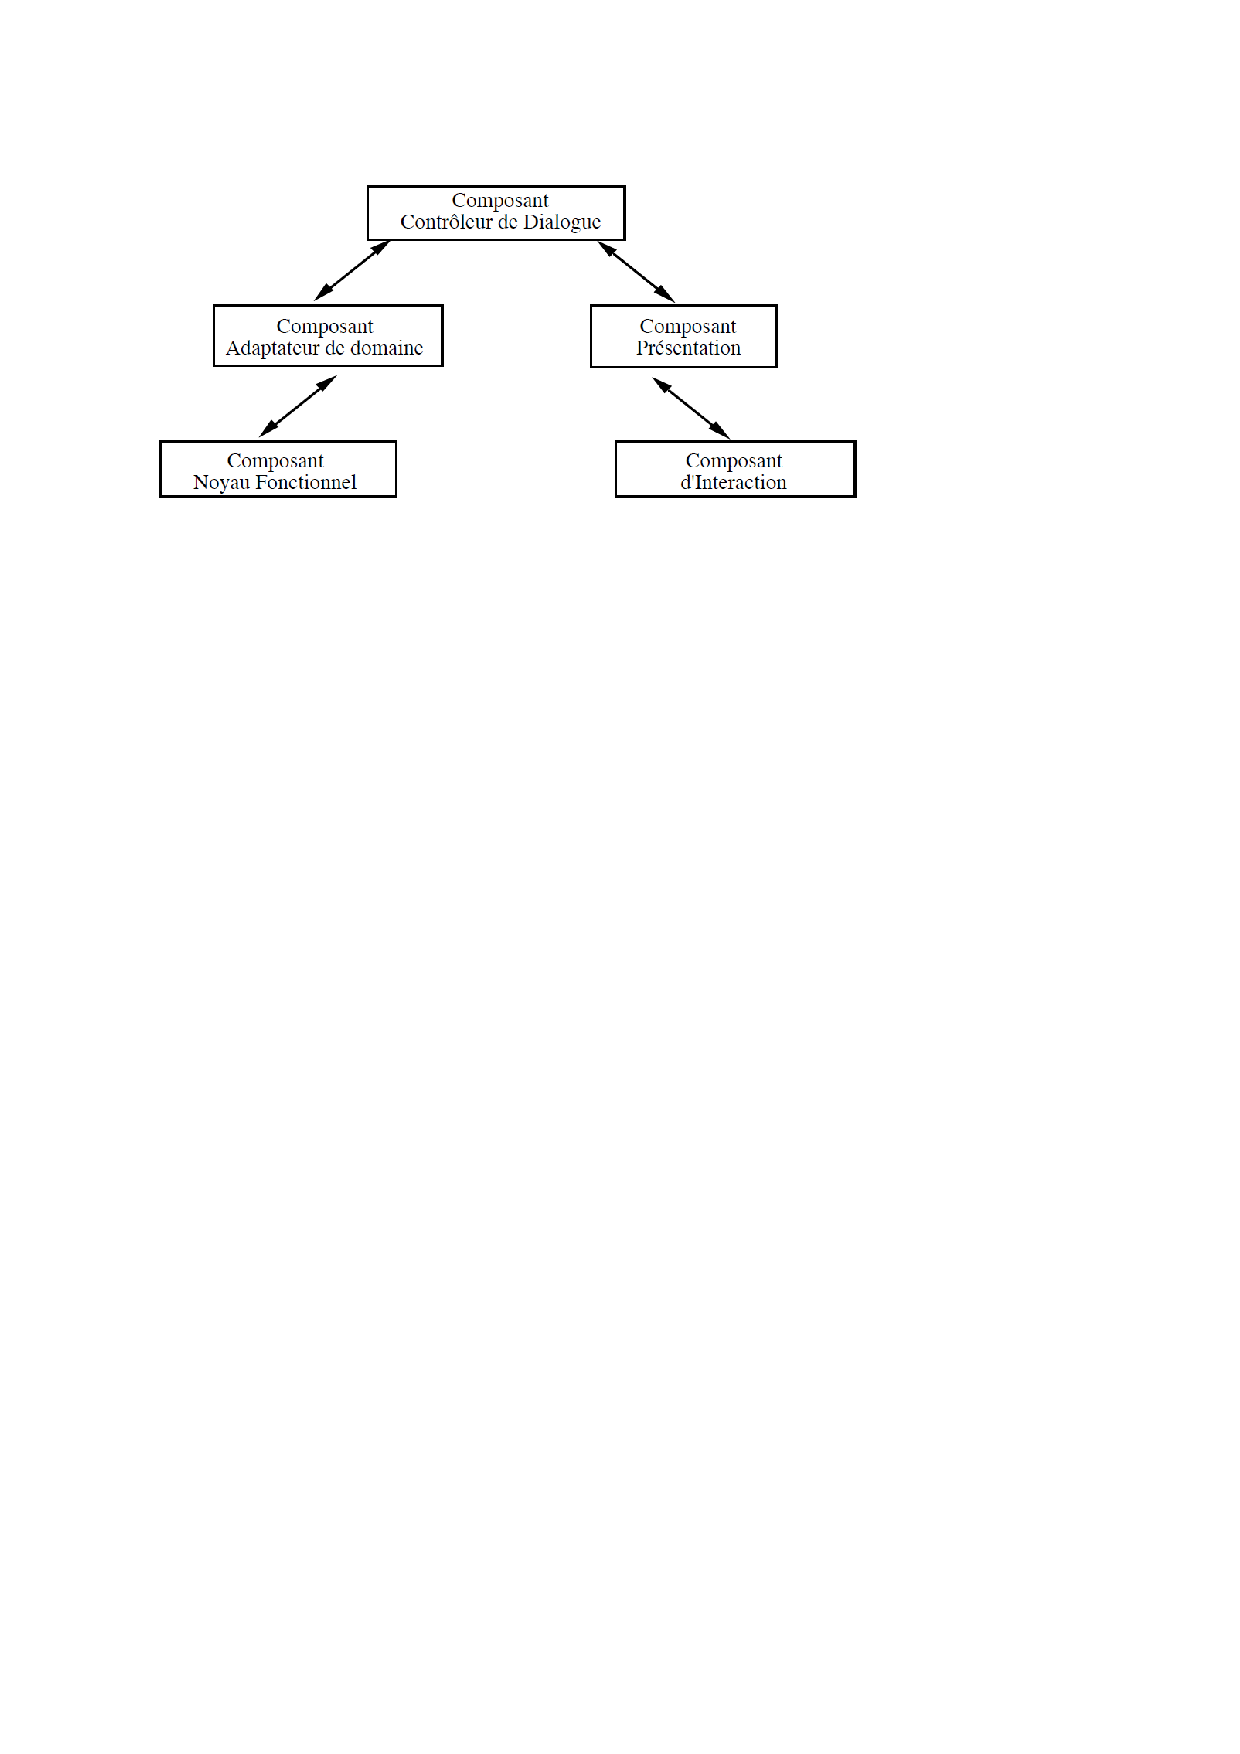
\includegraphics[scale=0.7]{chap3/img-9}
\end{center}
\end{figure}
\subsubsection{Processus de migration de l'UI}
Cette approche consiste à remplacer les composants des interacteurs logiques et physiques de l'UI à migrer pour qu'ils soient conformes aux principes de conception de la table interactive ciblée. Elle est proposée par Thevenin et al. ~\cite{Thevenin2002} pour résoudre le problème de la conception d'une IHM multi cible adaptable. Elle propose quatre niveaux d'adaptation : l'adaptation des interacteurs physiques, l'adaptation des interacteurs logiques, l'adaptation du contrôleur de dialogue et l'adaptation de l'adaptateur du NF. Pour la migration d'UI vers les tables interactives en conservant le NF de l'application de départ, l'on peut s'intéresser aux niveaux d'interacteurs physiques et logiques.

\paragraph{ Migration des interacteurs physiques}
Elle concerne l'adaptation du composant d'interaction  du modèle ARCH~\cite{Pfaff1985}, l'UI de l'application est portée sur la plateforme d'arrivée et utilise les objets de la boîte à outils présents sur la plateforme cible. Ce type d'adaptation permet de conserver la nature des composants graphiques mais leur rendu est distinct en fonction des plateformes et des  boîtes à outils. La figure \ref{fig:chap3:2} ci-dessous montre l'exemple de l'adaptation  d'un bouton physique lorsque le système est migré entre les plateformes MacOS-X, Java/JFC et PalmOS.

\begin{figure}[ht]
\begin{center}
\label{fig:chap3:2}
\caption{ Adaptation du niveau de l'interaction physique}
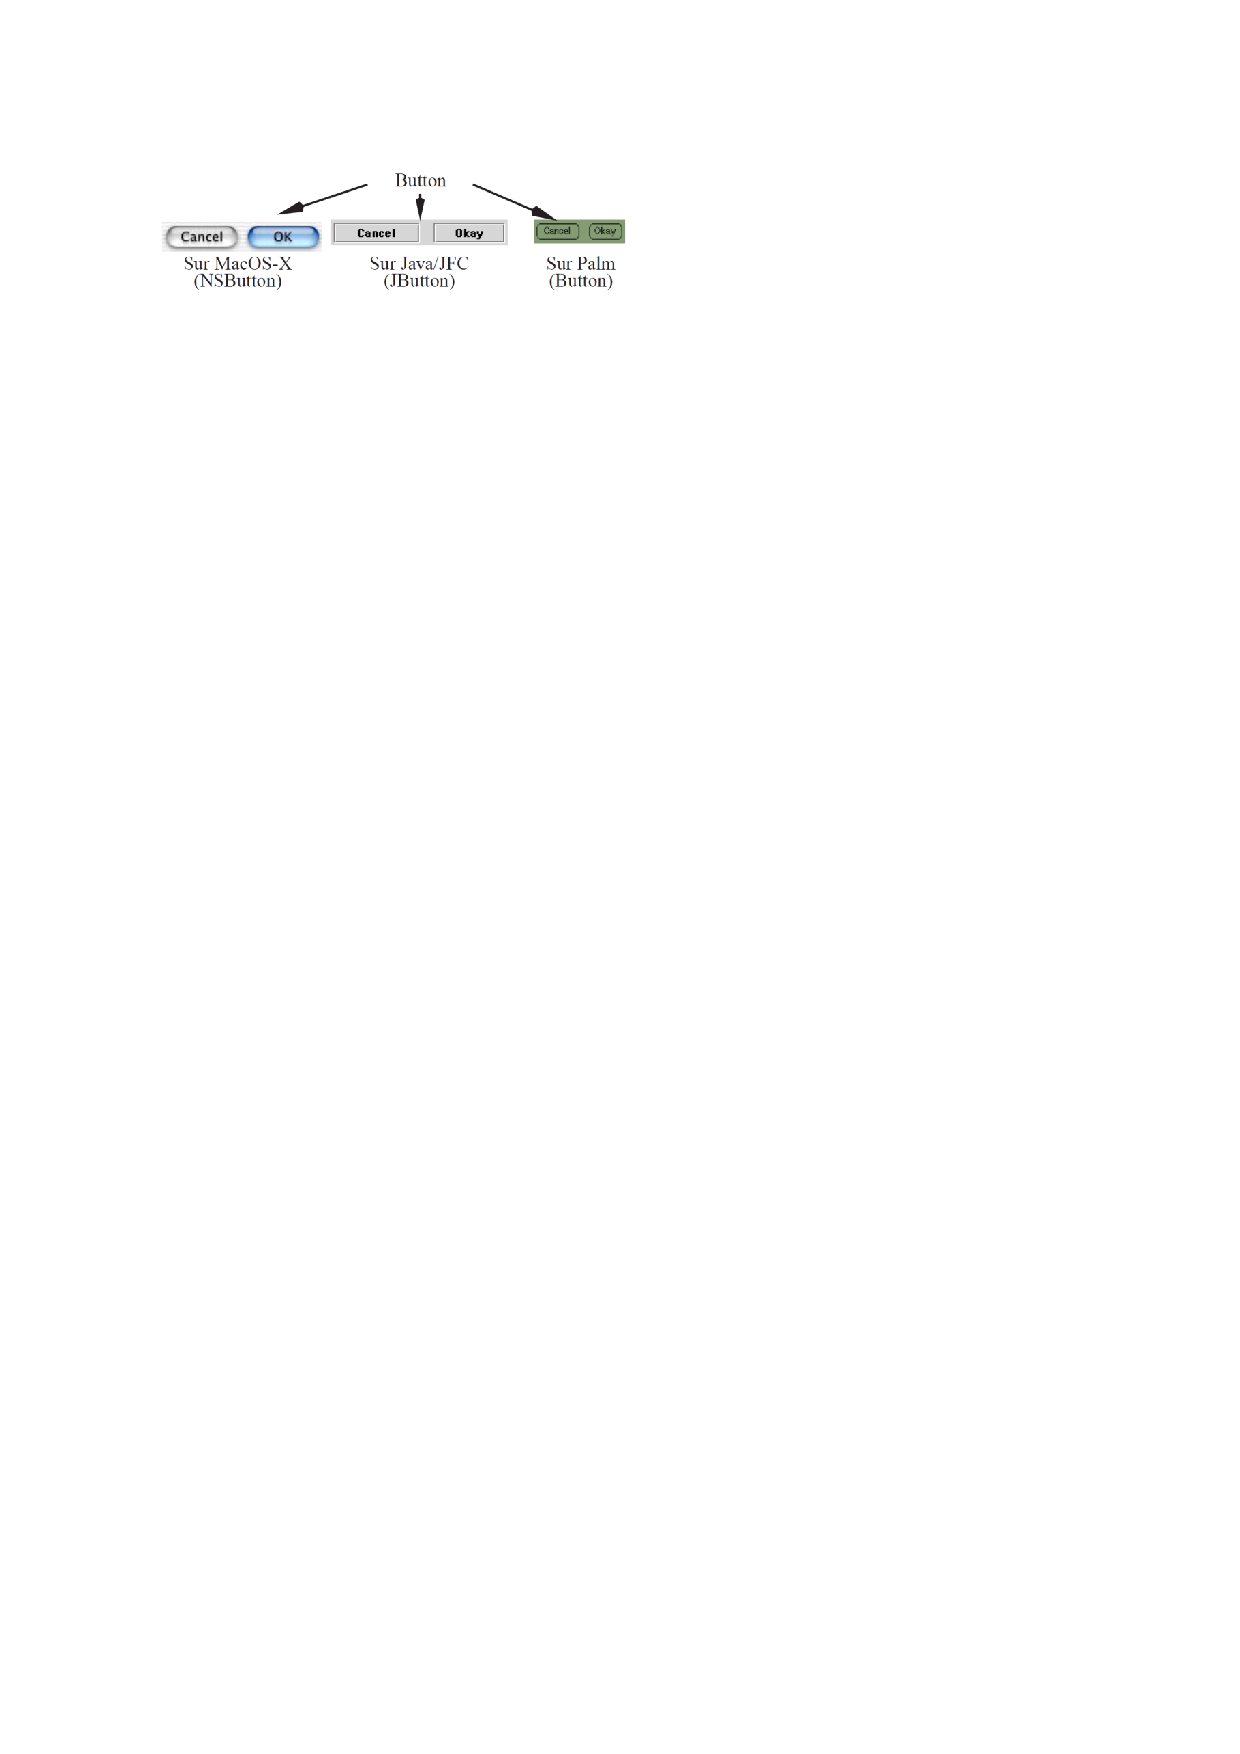
\includegraphics[scale=1]{chap3/img-3}
\end{center}
\end{figure}

Cette approche présente deux limites d'une part elle ne prend pas en compte la différence des modalités d'interactions entre les plateformes de départ et d'arrivée. En effet il y a une différence entre les modalités d'interactions d'un desktop et d'une table interactive(cf section %\ref{{sec:chap2:2:3}) 
. D'autre part ce type d'adaptation ne prend en compte les critères ergonomiques à liées à la plateforme d'arrivée. Cependant d'adaptation du niveau d'interaction permet de conserver les composants du NF, de l'adaptateur du NF, du contrôleur de dialogue et de la présentation.

\subsubsection{ Prise en comptes des principes de conception }
Elle concerne l'adaptation du composant de présentation du modèle ARCH~\cite{Pfaff1985}, l'UI de l'application est migrée sur la plateforme d'arrivée en changeant la représentation mais en conservant les fonctionnalités et la navigabilité. Avec ce type d'adaptation, les interacteurs sont de nature distinctes mais leur capacités représentationnelles et fonctionnelles sont équivalentes. Cette adaptation ne modifie pas le contrôleur de dialogue. La figure \ref{fig:chap3:3} ci-dessous montre le cas d'une liste de sélection (ComboBox) et d'une étiquette (Label) qui peuvent être remplacées par un champ de texte(TextField) et une étiquette (Label) ou par un composant graphique dédiée qui décrit les éléments de la liste avec des icones et du texte. 
\begin{figure}[ht]
\begin{center}
\label{fig:chap3:3}
\caption{Adaptation du niveau de la présentation logique}
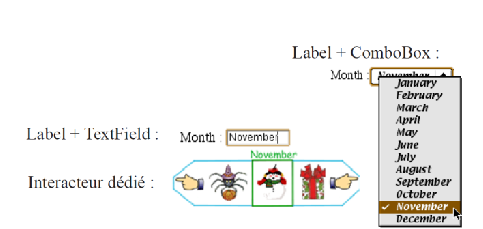
\includegraphics[scale=1]{chap3/img-4} 
\end{center}
\end{figure}
Dans le cadre de la migration vers la table interactive, cette adaptation permet de prendre en compte les critères ergonomiques de la plateforme, car à ce niveau il est possible de choisir des composants graphiques qui préservent les capacités représentationnelles, fonctionnelles et navigationnelles de l'UI de départ et qui respectent les critères ergonomiques. Par exemple l'interacteur dédié de la figure\ref{fig:chap3:3} est conseillé sur les tables interactives car il est préférable d'utiliser des images que des textes simples. Les capacités représentationnelles d'un interacteur logique sont le type des données qu'il contient et sa cardinalité, les capacités fonctionnelles sont l'ensemble des fonctionnalités accessibles à travers un interacteur et les capacités navigationnelles sont des tâches particulières qui facilitent l'accès et l'utilisation des autres composants graphiques. 
Dans l'objectif d'automatiser cette approche, il semble indispensable de pouvoir décrire les équivalences entre les interacteurs logiques en se basant sur un modèle qui décrit les capacités fonctionnelles, représentationnelles et navigationnelles de chaque interacteurs. Les composants de présentations sont décrits en utilisant des objets interactifs abstraits (OIA) et des objets interactifs concrets (OIC)~\cite{Vanderdonckt1993}.

\subsubsection{Résumé}
[Todo]

